 \section{Experiments}
 In this section, we empirically evaluate the effectiveness and efficiency of the proposed algorithms. First, we describe the baseline approaches and evaluation methodology of the experiments. We use two real-world LBSN datasets shown in Table IV. The \textit{FB} dataset is collected by Facebook API\footnote{Facebook Developers. https://developers.facebook.com/}. We have taken 96 volunteers' Facebook accounts as user seeds (most of the users live in Taiwan) and crawled all their and their friends' location records (i.e., check-ins and geo-tagged photos) over the period of Jan. 2012 - Dec. 2014. \textit{CA} is another Foursquare dataset with an undirected friendship network from~\cite{gao2012exploring}. All the experiments are conducted on an x86\_64 Linux server with 16 cores and 8 GB memory. %The \textit{GWL} dataset\footnote{Stanford Network Analysis Project (SNAP). http://snap.stanford.edu/data/loc-gowalla.html} and \textit{FS} are two check-in datasets with an undirected friendship network. Note that \textit{GWL} and \textit{FS} are larger datasets but lack with the information of POI categories.

\begin{table}[h]
\begin{center}
\caption{Details of the LBSNs}
\footnotesize{
\begin{tabular}{|l|c|c|c|}
  \hline
   & Property & \multicolumn{2}{|c|}{Network} \\ \cline{3-4}
   & & \textbf{FB} & \textbf{CA}\\
  \hline
   \#records & check-in & 869,317 & 483,813\\
  \hline
   \#nodes & user & 29,512 & 4,163\\
   & POI & 225,077 & 121,142\\
  \hline
   \#edge & friend & 39,513 & 32,512\\
  \hline
\end{tabular}}\\
\end{center}
\label{table:data.des}
\vspace{-1.3mm}
\end{table}

To gain insights into the datasets, we plot both the number of check-ins and routes of each user of our datasets. As shown in Figure~\ref{fig:exp_obs}, the number of check-ins and routes for each user is highly skewed in both datasets. Moreover, all distributions have long tails. In particular, the top 10\% ranked users in all datasets have nearly 60\% of total check-ins and routes. This indicates that most of the users are quite inactive. The data sparsity issue may cause considerable bias on the result of inactive users. So we chose the top 10\% of users, who were ranked by the travel route histories they have, as active users for testing. 
% 和沒有sample有何差別

\begin{figure}[h]
\centering
\mbox{
    \subfigure[Check-in distribution of \textit{CA} dataset]{
        \label{fig:exp_obs1}
        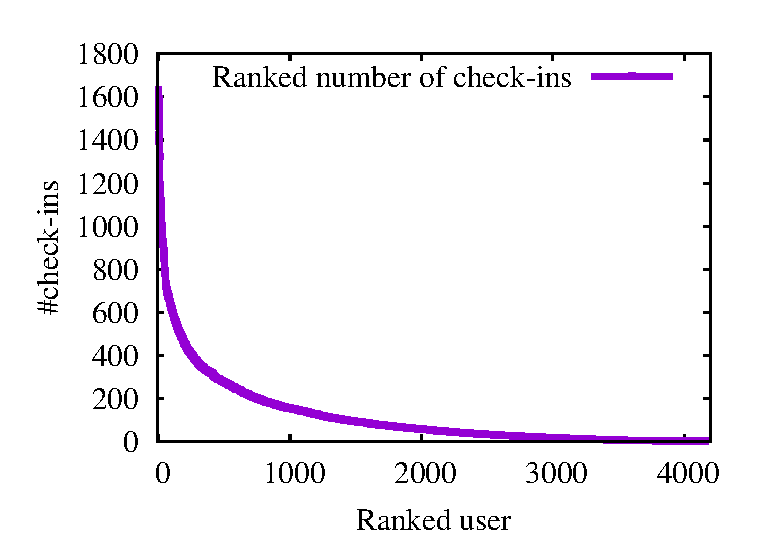
\includegraphics[width=0.48\linewidth]{obs_checkin_ca.eps}
    }
    \subfigure[Check-in distribution of \textit{FB} dataset]{
        \label{fig:exp_obs2}
        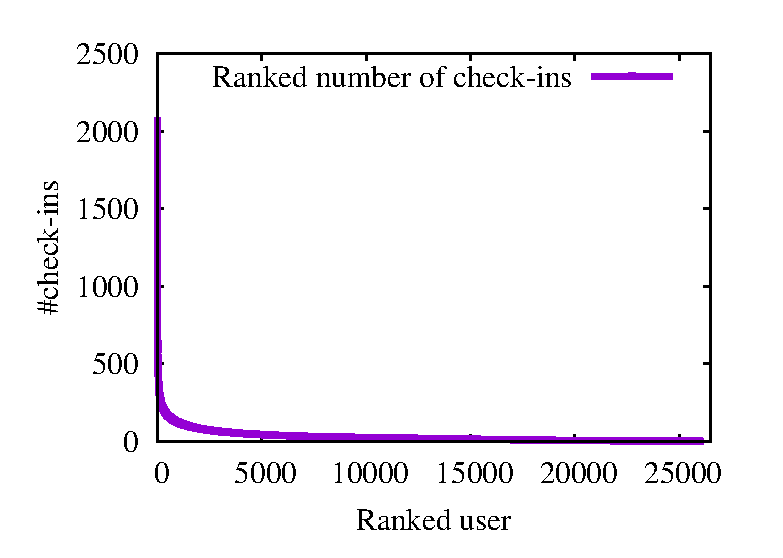
\includegraphics[width=0.48\linewidth]{obs_checkin_fb.eps}
    }
}
\mbox{
    \subfigure[Route distribution of \textit{CA} dataset]{
        \label{fig:exp_obs3}
        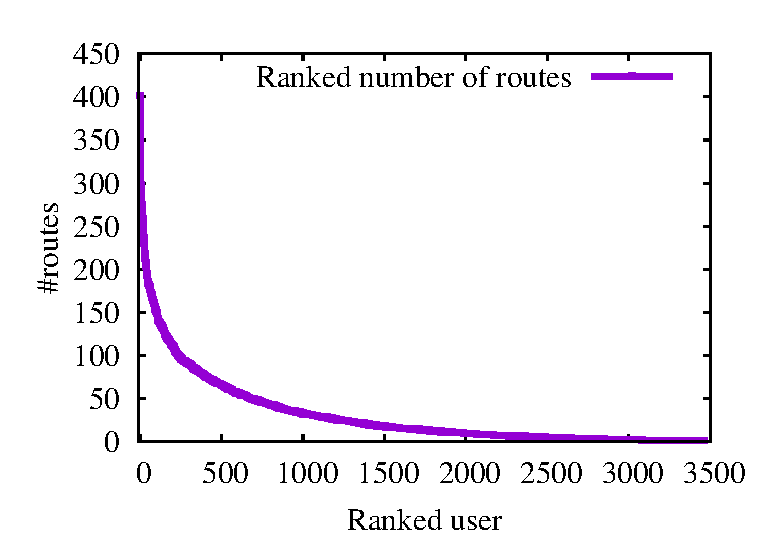
\includegraphics[width=0.48\linewidth]{obs_route_ca.eps}
    }
    \subfigure[Route distribution of \textit{FB} dataset]{
        \label{fig:exp_obs4}
        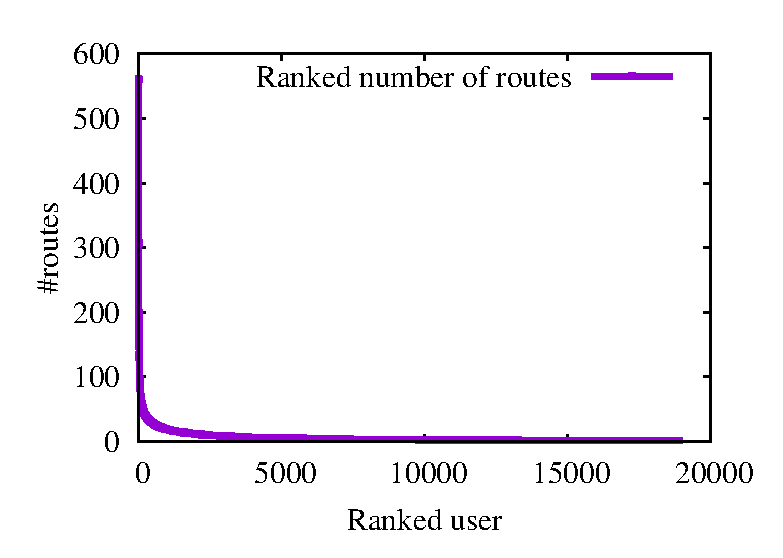
\includegraphics[width=0.48\linewidth]{obs_route_fb.eps}
    }
}
\caption{The number of check-ins and the number of routes for all uses in \textit{CA} and \textit{FB} dataset, respectively. The distribution shows a long tail extending in the negative direction.}
\label{fig:exp_obs}
\end{figure}

% \subsection{Keyword matching accuracy}
\subsection{Keyword matching accuracy} \label{sec:exp.keyword}

In this subsection, we evaluate the quality of the extracted keywords. Since our check-in datasets do not have sufficient text descriptions, i.e., tags, we collected an additional photo dataset consisting of 165,057 photos with 958,441 tags in the same local area. For that, the tags are regarded as input keyword. We ranked the tags by using scores in Section III-A and measured precision@$K$. Table V shows the precision of deciding  the Geo-specific, Temporal, and Attribute keywords.\footnote{For attribute extraction, we adopt~\cite{lee2013attribute} extracting probable attributes of all possible concepts. We can adopt 10 concepts aligned with POI categories, and Table VI illustrates attributes of `Food' concept for restaurant POIs.} We can see that the precision is reasonably high and does not decrease much as $K$ increases. Table VI shows the results for keyword extraction. Note that the keywords in italics are the Chinese keywords returned, which we translate for presentation. In the geo-specific dimension, 10 keywords referring to certain places are highly ranked. For example, a keyword `Longshan' represents `Longshan Temple'. In the temporal dimension, there is no doubt that keywords such as `Sunset', `Sunrise', `Lunch' and `Night' are specific to a certain time interval. `Dadaocheng' is ranked high as it is a place famous for its sunset. Also, `Butterfly' and `Fireworks' are strongly associated with day time and night time respectively. In the attribute dimension, keywords relevant to restaurant POIs are highly ranked.

\begin{table}[h]\scriptsize
\begin{center}
\caption{Precision of keyword extraction}
\vspace{1mm}
{\scriptsize\begin{tabular}{ | c | c | c | c |}
    \hline
     & P@10 & P@20 & P@40 \\ \hline\hline
    Geo-specific keyword &  1.000&  1.000& 0.975 \\ \hline
    Temporal keyword &  0.900&  0.700& 0.720 \\ \hline
    Attribute keyword & 1.000&  0.850& 0.775 \\ \hline
 \end{tabular}}
\end{center}
\label{tab:keywordex1}
\end{table} 
\vspace{-2mm}

\begin{table}[h]\scriptsize
\begin{center}
\caption{Top-10 results of keyword extraction}
\vspace{1mm}
{\scriptsize\begin{tabular}{ | c | p{24mm} | p{13mm}  | p{13mm} |}
    \hline
    & \multicolumn{3}{c|}{Keyword types} \\ 
    \cline{2-4}
     & \hspace{5mm} Geo-specific&\hspace{1mm}  Temporal &\hspace{1.5mm}  Attribute \\ \hline
    1 & Longshan &  \textit{Sunset}  & Recipe\\ \hline
    2 & \textit{Guanghua digital plaza} &  Sunset  & Soup \\ \hline
    3 & \textit{Huashan creative park} &  \textit{Sunrise}  & Store \\ \hline
    4 & \textit{NTN univ.} &  \textit{Dadaocheng}  & Oil \\ \hline
    5 & \textit{Dadaocheng dock} & \textit{Fireworks}   & Sale \\ \hline
    6 & \textit{Forty-four village}& Fireworks & Butter \\ \hline
    7 & \textit{Taipei fine arts museum} &  Butterfly   & Sauce \\ \hline
    8 & \textit{Three gorges street} & Boat   & Bread \\ \hline
    9 & Ximending & Lunch   & Chicken\\ \hline
    10 & \textit{CKS memorial hall} & Night  & Delivery \\ \hline
 \end{tabular}}
\end{center}
\label{tab:keywordex2}
\end{table}
\vspace{-2mm}

\subsection{Efficiency} \label{sec:exp_run_time}
Table VII shows the online response time of \textit{KSTR} in three main sub-procedures: (i) generate candidate routes (Reconstruct), (ii) compute the score of original/reconstructed routes (O\_scoring+R\_scoring), and (iii) Skyline search (Skyline). We synthesize 34,928 queries from testing users of \textit{FB} dataset and 39,729 queries from \textit{CA} dataset. The average response is 1.561708549 seconds. We can find that \textbf{Reconstruct} is the most time-consuming step. In Subsection~\ref{subsec:turing}, we observe the optimal $N$ for approximate candidate route generation. The total running time under different scales is shown in Subsection~\ref{subsec:scale}.

\begin{table}[h]\label{fig:exp_time}
\centering
\caption{Running time ratio (sub-procedure time cost / total time cost) of each step.}
\begin{footnotesize}
\begin{tabular}{|r|c|c|c|c|} \hline
 & \textbf{Reconstruct} & \textbf{O\_scoring} & \textbf{R\_scoring} & \textbf{Skyline} \\ \hline
\textbf{FB} & 0.265513757 & 0.160751505 & 0.040780763 & 0.099222254 \\ \hline
\textbf{CA} & 0.213114739 & 0.155153407 & 0.038816553 & 0.163912108 \\ \hline
\end{tabular}
\end{footnotesize}
\end{table}

\subsubsection{Tuning Approximate Parameters} \label{subsec:turing}
First, we study the accuracy of the approximate routes reconstruction algorithm. We define the term ``relative ratio'' as the ratio of reconstructed routes to the Skyline searched results. By randomly choosing 1,000 routes in the testing set, we observe the optimal parameter $N$ for selecting the top-$N$\% ranked POIs to generate routes that controls the best trade off between effectiveness and running time. Figure~\ref{fig:exp_approx} shows the average relative ratio of the 1,000 testing routes compared to the value of $N$. Note that the brute-force method is $N=100$. 

\begin{figure}[h]
\centering
\mbox{
    \subfigure[The relative ratio of reconstructed routes in \textit{CA} dataset]{
        \label{fig:exp_approx1_ca}
        \includegraphics[width=0.47\linewidth]{exp_approx1_ca.eps}
    }
    \subfigure[The relative ratio of reconstructed routes in \textit{FB} dataset]{
        \label{fig:exp_approx1_fb}
        \includegraphics[width=0.47\linewidth]{exp_approx1_fb.eps}
    }
}
\mbox{
    \subfigure[The running time of the reconstruction of the \textit{CA} dataset]{
        \label{fig:exp_approx2_ca}
        \includegraphics[width=0.47\linewidth]{exp_approx2_ca.eps}
    }
    \subfigure[The running time of the reconstruction of the \textit{FB} dataset]{
        \label{fig:exp_approx2_fb}
        \includegraphics[width=0.47\linewidth]{exp_approx2_fb.eps}
    }
}
\caption{The effectiveness of the candidate route generation of the \textit{CA} and \textit{FB} dataset, respectively under different top-$N$\% of POI elements. The results converge as $N$ increases.}
\label{fig:exp_approx}
\end{figure}

As shown in Figures~\ref{fig:exp_approx1_ca} and \ref{fig:exp_approx1_fb}, we can find that the relative ratio of both datasets converges rapidly as $N$ increases. Moreover, although the running time of reconstruction is only slightly longer when $N=100$, the running time of the whole procedure is obviously affected. The reason is that the number of generated routes increases exponentially w.r.t. the size of the POI elements. Moreover, the growth trend of route number levels off when $N>50$. Therefore, we choose $N=10$ in both datasets, which holds the accuracy and speed. % (level off)

\subsubsection{Scalability} \label{subsec:scale}
The objective of this set of experiments is to study the scalability of the proposed algorithms with variation of the number of computations. We have made use of several methods to optimize the implementation of the online system. Figure~\ref{fig:scalability} shows the total running time and the comparison of the sequential scoring and the multiprocess\footnote{Eight-cores multi-processing} scoring. In general cases, the number of route computations of a user query seldom exceeds 5,000 and the response time of the query takes no more than one second. Since the result is sufficiently fast, the multiprocess mechanism does not lead to evident improvement. On the other hand, in extreme cases with 26,000 route computations, using multiprocess reduces 25\% of time cost.

% \begin{table} \label{fig:scalability}
% \centering
% \caption{Runtime versus route number (computation size).}
% \begin{footnotesize}
% \begin{tabular}{|r|c|c||c|c|} \hline
% route \# & CA\_multi & CA\_seq & FB\_multi & FB\_seq \\ \hline
% 100 & 0.202882027626 & 0.0539593935013 & 0.224622035027 & 0.0833256959915 \\ \hline
% 200 & 0.169521689415 & 0.0586039066315 & 0.188808059692 & 0.0776352882385 \\ \hline
% 400 & 0.204951334 & 0.124091458321 & 0.251364135742 & 0.197812461853 \\ \hline
% 800 & 0.279544639587 & 0.230948734283 & 0.391712117195 & 0.38260076046 \\ \hline
% 1600 & 0.426859116554 & 0.471332502365 & 0.801701116562 & 0.72469959259 \\ \hline
% 3200 & 0.899803447723 & 0.939165329933 & 0.991176962852 & 1.19409227371 \\ \hline
% 6400 & 1.47143003941 & 1.85361101627 & 1.89424002171 & 2.25203275681 \\ \hline
% 12800 & 2.99047272205 & 3.77915635109 & 4.5547088623 & 4.68398189545 \\ \hline
% 25600 & 6.00035352707 & 7.98866209984 & 7.78471326828 & 9.47318651676 \\ \hline
% \end{tabular}
% \end{footnotesize}
% \end{table}
\begin{figure}[h]
\centering
\mbox{
    \subfigure[The relative ratio of reconstructed routes in the \textit{CA} dataset]{
        \label{fig:exp_effi_ca}
        \includegraphics[width=0.47\linewidth]{exp_effi_ca.eps}
    }
    \subfigure[The relative ratio of reconstructed routes in the \textit{FB} dataset]{
        \label{fig:exp_effi_fb}
        \includegraphics[width=0.47\linewidth]{exp_effi_fb.eps}
    }
}
\caption{Runtime versus route number (computation size).}
\label{fig:scalability}
\end{figure}

\subsection{Evaluation of route prediction accuracy}
In this experiment, we compared the following four baseline recommendation models to our keyword-aware skyline travel route (\textit{KSTR}) model.

\begin{figure*}[t]
\centering
\mbox{
    \subfigure[Average edit distance versus to recommended travel routes of \textit{FB} dataset]{
        \label{fig:exp_accuracy3_fb}
        \includegraphics[width=0.33\linewidth]{exp_prediction1_fb.eps}
    }
    \subfigure[Average region cover ratio versus to recommended travel routes of \textit{FB} dataset]{
        \label{fig:exp_accuracy2_fb}
        \includegraphics[width=0.33\linewidth]{exp_prediction2_fb.eps}
    }
    \subfigure[Average category similarity versus to recommended travel routes of \textit{FB} dataset]{
        \label{fig:exp_accuracy1_fb}
        \includegraphics[width=0.33\linewidth]{exp_prediction3_fb.eps}
    }
}
\mbox{
    \subfigure[Average edit distance versus to recommended travel routes of \textit{CA} dataset]{
        \label{fig:exp_accuracy1_ca}
        \includegraphics[width=0.33\linewidth]{exp_prediction1_ca.eps}
    }
    \subfigure[Average region cover ratio versus to recommended travel routes of \textit{CA} dataset]{
        \label{fig:exp_accuracy2_ca}
        \includegraphics[width=0.33\linewidth]{exp_prediction2_ca.eps}
    }
    \subfigure[Average category similarity versus to recommended travel routes of \textit{CA} dataset]{
        \label{fig:exp_accuracy3_ca}
        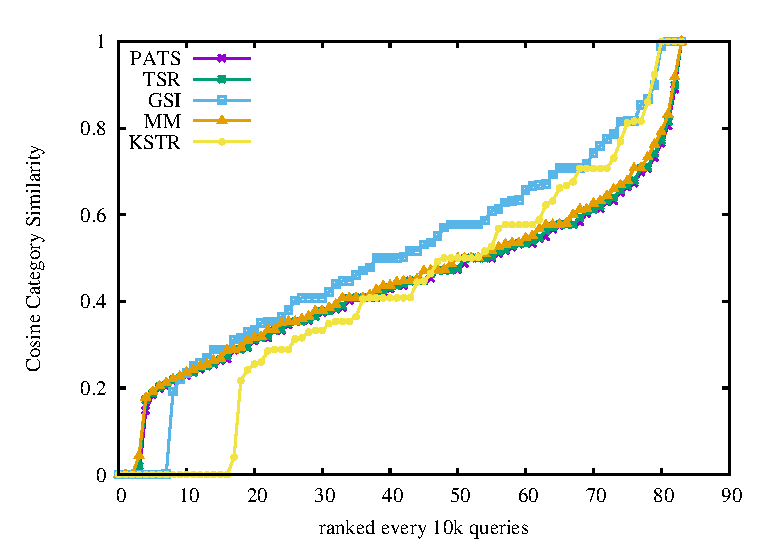
\includegraphics[width=0.33\linewidth]{exp_prediction3_ca.eps}
    }
}
\caption{Average goodness accuracy of recommended travel route at different query region sizes. The yellow line represents our method and shows that KSTR has the good results over the three measurements.}
\label{fig:exp_accuracy}
\end{figure*}

%\textbf{OSScaling model:}
%~\cite{cao2012keyword} outputs the travel routes based on the user’s interests, which is calculated by the Markov model P(lt|lt−1). The most chosen landmark, given the current landmark, is always recommended. This model considers the user’s current location but does not consider the user’s interest.

%\textbf{Markov-Topic model:}
%~\cite{kurashima2010travel} outputs the next route based on the user’s current location and interest, which is calculated by combining the Markov model and the topic model using the unigram rescaling technique.

\noindent\textbf{Pattern aware trajectory search (PATS):}
Only consider the sum of the POI attractiveness score. Different to the Multinomial model, \cite{PATS} consider the mobility transition among POI pairs.

\noindent\textbf{Time-sensitive routes (TSR):}
Only consider the visiting time score of routes. The arrival time of the POIs in the recommendation best fits the extracted proper visiting time.

\noindent\textbf{Geo-social influenced routes (GSI):}
Only consider the geo-social influence score of \cite{ytwen2014}. The route consists of POIs visited by geo-social influential users in social network.

\noindent\textbf{Multinomial model (MM):} 
This is the naive method that outputs the travel routes based on all three features. Routes are ranked by the summation of the feature scores. % r!!! evised

\noindent\textbf{Keyword-aware skyline route (KSTR):}
\textit{KSTR} outputs diverse Skyline routes based on both POI and user factors.

Unfortunately, raw LBSN data provide no ground truth to verify the acceptance of the recommended travel route suggestions. Therefore,
we studied the ``appropriateness'' of the recommended travel routes as a route prediction progress under different spare time conditions. We used the data shown in Table IV for training and testing the model. For each dataset, the test data were created by collecting the last travel sequence of the top-10\% of users (ranked by route count) in the most recent $30$\% time periods. The training dataset consisted of the set of travel sequences excluding the testing data part. To be exact, the number of training data (the number of test data) used in this experiment is slightly larger than the number of testing data since users with multiple travel sequences only keep the last sequence. 
% In order to evaluate the goodness of our method of adding query points into existing trajectories, we remove one ROI from each existing trajectory as a query point and then use our method to aggregate the removed ROI back into the trajectories. We call hit if the order of ROIs in the trajectories after aggregating the query point by our method is the same as the original trajectory order, as it indicates that the order is appropriate because there exists history trajectories that someone visited the ROI in the same order. The hit rate of our method in this experiment is about 69\%.

\subsubsection{Comparison of route prediction accuracy}
We measured the difference between the generated routes and each test sequence. Three goodness functions are applied as the evaluation metrics.

\noindent\textbf{Edit distance:} 
The edit distance measures the distance between two sequences in terms of the minimum number of edit operations required to transform one sequence into the other~\cite{kurashima2010travel}. The allowable edit operations are: insert into a sequence, delete from a sequence, and replace one landmark with another.

\noindent\textbf{Geographical region cover ratio:}
The test route and recommended route both can be bounded by a geographical box. The ratio of the overlapped region to the testing route region.

\noindent\textbf{Category similarity:}
To consider the closeness of user interest, we compute the cosine similarity of the categories between two routes, which is \textit{\# of overlapped category} / $\sqrt{\textit{\# of category1}\cdot\textit{\# of category2} }$.

We compared our \textit{KSTR} model with the other models: multinomial model, pattern aware trajectory search, time-sensitive and geo-social influenced routes. Figure~\ref{fig:exp_accuracy} shows the performance of each model among the three measures. We can find that the proposed \textit{KSTR} model offers the lowest edit distance, which represents the highest prediction accuracy. On the other hand, considering the measure of region cover ratio and category similarity, the multinomial model has better performance than ours. The results show that the proposed \textit{KSTR} is effective and beats other baselines and state-of-the-art methods in terms of route prediction accuracy. % !!! add ore descriptions We also tested the statistical significance of the difference between the average edit distances of the proposed and the baselines using the Wilcoxon signed-rank test. For each region, bandwidth, and spare time condition, the result of the Wilcoxon signed-rank test is p < 0.05 (two-sided test).

% \subsubsection{Running time comparison} \label{sec:exp_run_time}

\subsection{Examples of Route Recommendation: }
As a result, we implemented our proposed methods and constructed a web-based travel route recommender system. One example of recommended routes by the system is show.
\vspace{-1.5mm}

\begin{figure}[h]
\centering
\includegraphics[width=\linewidth]{exp_example2.eps}
\vspace{-7mm}
\caption{Examples of KSTR routes in Kaohsiung.}
\label{fig:example1} % 一定要在 caption 之後
\end{figure}

\vspace{-1.5mm}

Figure~\ref{fig:example1} shows the recommendation examples when the user gives a geographical region of Kaohsiung on the map interface and specifies a one day tour and  keywords [``Si Zih Bay'' ``Cuisine'']. The system provides five different trip plans. Note that, unlike ranking, the ordering of skyline results does not reflect relevance. \textit{Route \#4} is visualized on the map interface and each icon on the map represents a POI. Besides the specific region ``Si Zhi Bay'', ``Guo Ji meat dumpling'' and ``ShanMinng TeaShop'' are perfectly associated with the keyword ``Cuisine''. And we can see the route with the best visiting time suggestions.

\vspace{-3mm}